\documentclass[11pt]{article}

\usepackage[margin=1in]{geometry}
\usepackage{microtype}
\usepackage{lmodern}
\usepackage[T1]{fontenc}
\usepackage{amsmath,amssymb,amsthm,mathtools}
\usepackage{booktabs}
\usepackage{graphicx}
\usepackage{xcolor}
\usepackage[numbers,sort&compress]{natbib}
\usepackage[colorlinks=true,citecolor=blue,linkcolor=blue,urlcolor=blue]{hyperref}
\usepackage{algorithm}
\usepackage{algorithmic}
\usepackage{enumitem}
\usepackage{multirow}
\usepackage{array}
\usepackage{caption}
\usepackage{subcaption}
\usepackage{longtable}
\usepackage{parskip}
\title{Adversarial Latent-State Training for Robust Policies in Partially Observable Domains}
\author{
  Angad Singh Ahuja \\
  Constrained Image-Synthesis Lab
}
\date{\today}

\newtheorem{definition}{Definition}
\newtheorem{theorem}{Theorem}
\newtheorem{lemma}{Lemma}
\newtheorem{proposition}{Proposition}
\newtheorem{corollary}{Corollary}
\newtheorem{remark}{Remark}

\newcommand{\A}{\mathcal{A}}
\newcommand{\Sset}{\mathcal{S}}
\newcommand{\Oset}{\mathcal{O}}
\newcommand{\T}{\mathcal{T}}
\newcommand{\R}{\mathcal{R}}
\newcommand{\Zset}{\mathcal{Z}}
\newcommand{\Bset}{\mathcal{B}}
\newcommand{\Hset}{\mathcal{H}}
\newcommand{\Pset}{\mathcal{P}}
\newcommand{\E}{\mathbb{E}}
\newcommand{\Prob}{\mathbb{P}}
\newcommand{\tauT}{\tau}
\newcommand{\rhoNom}{\rho_{\mathrm{nom}}}
\newcommand{\rhoStress}{\rho_{\mathrm{stress}}}
\newcommand{\rhoU}{\rho_{\mathrm{U}}}
\newcommand{\rhoD}{\rho_{\mathrm{D}}}
\newcommand{\Gap}{\Delta_{\mathrm{rob}}}
\newcommand{\cvar}{\mathrm{CVaR}}
\newcommand{\gammaTrain}{\gamma_{\mathrm{train}}}
\newcommand{\TODO}[1]{\textbf{TODO: #1}}

\begin{document}
\maketitle

\begin{abstract}
Robustness under latent distribution shift remains challenging in partially observable reinforcement learning. We formalize a focused setting where an adversary selects a hidden initial latent distribution before the episode, termed an adversarial latent-initial-state POMDP. Theoretically, we prove a latent minimax principle, characterize worst-case defender distributions, and derive approximate best-response inequalities with finite-sample concentration bounds that make the optimization and sampling terms explicit. Empirically, using a Battleship benchmark, we demonstrate that targeted exposure to shifted latent distributions reduces average robustness gaps between Spread and Uniform distributions from $10.3$ to $3.1$ shots at equal budget. Furthermore, iterative best-response training exhibits budget-sensitive behavior that is qualitatively consistent with the theorem-guided diagnostics once one accounts for discounted PPO surrogates and finite-sample noise. Ultimately, we show that for latent-initial-state problems, the framework yields a clean evaluation game and useful theorem-motivated diagnostics while also making clear where implementation-level surrogates and optimization limits enter. The code repository for this work is available at \url{https://github.com/AngadSingh22/adversarial_pomdp}.
\end{abstract}

\section{Motivation and Claim}

Many partially observable control problems are dominated not by stepwise stochasticity, but by a hidden condition selected before interaction begins. A diagnosis system may face an unknown fault configuration. A robotics policy may confront an unobserved physical parameter regime. A constrained graphics system may act under a fixed but hidden process condition such as dot gain, substrate behavior, or capture distortion. In each case, the agent interacts sequentially, but the principal source of uncertainty is a latent variable drawn at the start of the episode and then held fixed.

This paper studies that setting through a deliberately restricted adversarial lens. The adversary does not modify transitions online and does not inject arbitrary trajectory-level noise. It acts only once, at time $0$, by choosing the hidden initial latent state or a distribution over such latent states. We refer to this problem class as \emph{adversarial latent-initial-state POMDPs}. Battleship is a particularly clean benchmark for this class. The hidden ship layout is exactly the latent variable. Conditional on the layout, transitions and observations are deterministic. The action space is discrete and constrained in a transparent way by already-fired cells. Strong scripted baselines are available. Most importantly, the hidden placement distribution can be varied in controlled ways to induce latent distribution shift.

The central claim of the paper has two parts. The first is theoretical. Adversarial latent-initial-state POMDPs admit a compact theorem package that is both exact and practically interpretable: the defender's optimization is a genuine finite minimax problem over latent distributions; approximate best responses imply explicit inequalities for the main training diagnostics; and finite-sample concentration guarantees certify when empirical signs of those diagnostics can be trusted. The second part is empirical. In Battleship, training exposure to shifted latent distributions substantially reduces robustness gaps under held-out stress distributions. However, full iterative best response only behaves as intended when the defender is itself optimized strongly enough to be genuinely adversarial.

The present benchmark is also motivated, in a modest way, by a broader graphics-for-ML agenda. In constrained image synthesis and sequential graphics control problems, one often faces hidden physical or process latents that remain fixed throughout a generation trajectory. Although this paper does not study those domains directly, the formal development is meant to be reusable there. Battleship is used here because it makes the latent-state structure exact and the theoretical analysis verifiable.

\section{Related Work}

The closest classical background is robust Markov decision process theory, where uncertainty typically enters through transition kernels or rewards and the control objective becomes minimax optimization over a model uncertainty set \citep{iyengar2005robust,nilim2005robust}. That literature is foundational, but its uncertainty model differs from the one studied here. In our setting, the adversary does not alter transition kernels throughout the episode. Instead, it selects a hidden initial latent condition, after which the environment evolves conditionally on that latent. This restriction is not merely cosmetic. It yields a simpler strategic object and, as we show, a cleaner theorem package.

Adversarial reinforcement learning has also been studied in forms where the adversary acts throughout the trajectory. Representative examples include robust adversarial reinforcement learning with a disturbance player \citep{pinto2017robust}, as well as broader lines of work on adversarial observations, adversarial state perturbations, and online disturbance robustness. These approaches are important and practically relevant, but they are structurally different from hidden-latent robustness. In those settings, the adversary is a trajectory-level controller. In the present paper, the adversary is a selector of initial latent conditions.

Partially observable sequential decision-making is naturally framed using POMDPs \citep{kaelbling1998pomdp}. In a general POMDP, the canonical sufficient statistic for optimal control is the posterior belief over hidden states. That perspective matters here because Battleship is fundamentally a search-under-uncertainty problem. It also explains why belief-style scripted baselines are so strong in this benchmark: they approximate posterior occupancy over hidden layouts. Our contribution, however, is not a new posterior filter or a new search baseline. It is a theorem-backed way of thinking about robustness when the hidden variable itself is adversarially chosen.

Closer structural relatives include planning problems with static hidden parameters and robust POMDP formulations with ambiguity over latent model components \citep{chen2016pomdplite,osogami2015robust}. Our setting is narrower than a general robust POMDP because the defender acts only once by choosing a latent initial condition. That restriction is deliberate: it isolates a hidden-latent subclass in which the defender strategy space, the relevant robustness gaps, and the diagnostic quantities all become especially transparent.

On the optimization side, we use PPO \citep{schulman2017ppo} together with action masking. This is a natural choice in Battleship because invalid actions are rule-defined rather than learned. For evaluation, we use not only mean episode length but also tail metrics such as the $95^{\text{th}}$ percentile and conditional value-at-risk \citep{rockafellar2000cvar,chow2015cvar}. This is important because robustness failures under latent shift often appear first in the tails rather than in the mean.

The game-theoretic training protocol is related to fictitious play and iterative best-response ideas \citep{brown1951fictitious,heinrich2016fsp}. However, our defender is intentionally restricted. It does not act as an unrestricted online adversary, nor does it directly optimize over all legal layouts in one step. It learns within a structured latent-selection class and is then evaluated through the induced distribution over layouts. This restricted viewpoint is central to the empirical story: the theoretical diagnostics are meaningful precisely because the defender's role is mathematically clear, but their empirical success depends on whether that restricted defender can be optimized well enough to behave adversarially in practice.

Finally, the present work should be read as part of a broader methodological tendency in machine learning toward robustness under hidden nuisance variation. Domain randomization and stress-distribution training pursue a related intuition, namely that controlled exposure to variation can improve out-of-distribution performance. The present paper differs in two ways. First, the latent variable is hidden and fixed rather than directly observed or resampled within an episode. Second, the main contribution is not simply an empirical robustness gain, but a mathematically explicit set of statements connecting the game formulation, the training objectives, and the diagnostics used to interpret them.

\section{Methodology, Theoretical Development, and Diagnostics}

The problem formulation and the methodological choices are best presented together. The formal game specifies the hidden latent layout, the observation channel, the feasible action set, and the objective. The solution space then specifies how that game is operationalized in learning: the reward surrogate used during optimization, the policy class actually implemented, the self-play protocol, and the evaluation quantities that connect the experiments back to the theory.

Let the board be an $H\times W$ grid. In the implementation and in the analysis below, cells are indexed as
\[
\mathcal{C}=\{0,1,\dots,HW-1\}.
\]
A legal hidden ship layout is an element $B\in\Bset$, where $\Bset$ is the finite set of all placements satisfying the standard legality constraints. The latent layout is treated as hidden because the attacker never observes ship locations directly. Instead it receives only immediate shot outcomes: miss, hit, or a sunk event for a specific ship. This is the minimum information required to preserve the actual information structure of the game. The underlying state at time $t$ may be written as
\[
s_t=(B,M_t,H_t,U_t),
\]
where $M_t$ and $H_t$ denote the public miss and hit indicators and $U_t$ denotes the remaining unsunk ship structure. The action set consists of valid grid cells not yet fired upon,
\[
\A(s_t)=\{a\in\mathcal{C}: M_t(a)=0 \wedge H_t(a)=0\}.
\]
Conditioned on $B$, the environment is deterministic. The only randomness under standard play enters through the initial layout draw.

\begin{definition}[Battleship POMDP]
A Battleship episode is a POMDP
\[
\mathcal{M}=(\Sset,\A,\Oset,\T,\Omega,\R)
\]
such that a hidden layout $B$ is sampled once at time $0$ and then fixed; the public state evolves deterministically through the hit, miss, and sunk updates; the observation kernel $\Omega$ is deterministic conditional on the hidden layout and public shot record; and the default reward is a step penalty until all ships are sunk.
\end{definition}

The natural performance criterion is shots-to-win. Let $\tauT$ denote the first time all ships are sunk. The game-level objective is
\[
\min_{\pi}\E_{\pi}[\tauT].
\]
All main theorems below are stated for this evaluation loss, because $\E_{\pi}[\tauT]$ is the quantity reported throughout the empirical section. The following lemma explains the exact relation between shots-to-win and the sparse step-penalty reward in the undiscounted setting.

\begin{lemma}[Undiscounted step penalty and shots-to-win]
Suppose the reward is
\[
r_t=-1 \quad \text{for } t<\tauT, \qquad r_{\tauT}=0.
\]
Then for any policy $\pi$,
\[
J_1(\pi):=\E_{\pi}\left[\sum_{t=0}^{\tauT-1}r_t\right] = -\E_{\pi}[\tauT].
\]
Therefore maximizing undiscounted expected return is exactly equivalent to minimizing expected shots-to-win.
\end{lemma}

\begin{remark}[Discounted PPO surrogate in the implementation]
The Stage-1 and Stage-2 PPO agents in the code are trained with discount factor $\gammaTrain=0.99$. For the sparse step-penalty reward, the resulting optimization objective is
\[
J_{\gammaTrain}(\pi)
:=
\E_{\pi}\left[\sum_{t=0}^{\tauT-1}\gammaTrain^t r_t\right]
=
-\E_{\pi}\left[\frac{1-\gammaTrain^{\tauT}}{1-\gammaTrain}\right].
\]
This discounted surrogate is monotone in $\tauT$ on each realized trajectory but is not equal to $-\E_{\pi}[\tauT]$ in expectation. The theorem package below should therefore be read as characterizing the evaluation game defined by episode length, while PPO serves as an optimization method for a closely related discounted surrogate.
\end{remark}

The exact POMDP sufficient statistic is the posterior belief over legal layouts,
\[
b_t(B)=\Prob(B\mid h_t),
\]
where $h_t$ denotes the interaction history up to time $t$. In principle, optimal control could be stated entirely in belief space. In practice, the implemented agents do not maintain that posterior explicitly. Instead, they receive a public board record encoded as a three-channel tensor with channels Hit, Miss, and Unknown, where Unknown is computed deterministically as
\[
\textsf{Unknown}=1-(\textsf{Hit}+\textsf{Miss}).
\]
This design is faithful to the implementation and keeps the policy class computationally tractable. Conceptually, however, the posterior remains important: it explains why belief-based baselines are strong and why the hidden-latent view of the game is the correct one.

The formal extension that matters for robustness is now immediate.

\begin{definition}[Adversarial latent-initial-state POMDP]
An adversarial latent-initial-state POMDP is a POMDP in which a latent variable $z\in\Zset$ is sampled once at time $0$ from a defender-chosen distribution $\rho$, after which the transition and observation laws remain fixed conditional on $z$, and the attacker acts under partial observability to optimize expected return.
\end{definition}

Battleship instantiates this definition exactly, with $z=B\in\Bset$. The defender's strategic role is therefore not to perturb the agent online, but to choose a hidden initial condition that changes the induced difficulty distribution over episodes.

For any loss variable $X$ under defender distribution $\rho$, write
\[
p95_{\rho}(X)
:=
\inf\{x\in\mathbb{R}: \Prob_{\rho}(X\le x)\ge 0.95\},
\]
and
\[
\cvar_{0.10,\rho}(X)
:=
\frac{1}{0.10}\int_{0.90}^{1}F^{-1}_{X,\rho}(u)\,du,
\]
so that $\cvar_{0.10,\rho}$ is the mean of the worst $10\%$ upper tail when $X$ is interpreted as a loss.

We measure robustness relative to a nominal defender distribution $\rhoNom$ and a stress defender distribution $\rhoStress$. For an attacker policy $\pi$, the mean robustness gap is
\[
\Gap(\pi)=\E_{\rhoStress}[\tauT(\pi)]-\E_{\rhoNom}[\tauT(\pi)].
\]
We also use tail-sensitive analogues,
\[
\Gap^{(p95)}(\pi)=p95_{\rhoStress}(\tauT(\pi))-p95_{\rhoNom}(\tauT(\pi)),
\]
and
\[
\Gap^{(\cvar)}(\pi)=\cvar_{0.10,\rhoStress}(\tauT(\pi))-\cvar_{0.10,\rhoNom}(\tauT(\pi)).
\]
These quantities match the evaluation protocol actually used in the experiments.

At this point the main theorem package can be stated. The first result is the central mathematical claim of the paper. Because the horizon, action set, and observation set are finite in Battleship, the set of deterministic history-dependent attacker policies is finite, although large. This permits an exact reduction of the attacker-defender interaction to a finite zero-sum game.

\begin{definition}[Deterministic history-dependent attacker policy]
Let $\Hset$ be the finite set of all feasible attacker histories up to a finite horizon $T_{\max}$. A deterministic history-dependent attacker policy is a map
\[
\pi:\Hset\to\mathcal{C}
\]
such that $\pi(h)\in\A(h)$ for every feasible history $h\in\Hset$.
\end{definition}

Let $\Pi^{\det}$ denote the finite set of all such deterministic attacker policies. Let the defender class be a compact convex polytope
\[
\Pset=\mathrm{conv}\{\rho^1,\dots,\rho^m\}
\]
of admissible latent distributions over a finite latent set $\Zset$. For each $\pi\in\Pi^{\det}$ and each latent $z\in\Zset$, define the latent-conditioned loss
\[
L(\pi,z):=\E[\tauT(\pi)\mid z].
\]

\begin{theorem}[Latent minimax principle]
Assume that the horizon $T_{\max}$ is finite, the action and observation alphabets are finite, the latent set $\Zset$ is finite, and the defender class $\Pset$ is a compact convex polytope of latent distributions. Then:
\[
\min_{\mu\in\Delta(\Pi^{\det})}\max_{\rho\in\Pset}V(\mu,\rho)
=
\max_{\rho\in\Pset}\min_{\mu\in\Delta(\Pi^{\det})}V(\mu,\rho),
\]
where
\[
V(\mu,\rho)=\sum_{\pi\in\Pi^{\det}}\sum_{z\in\Zset}\mu(\pi)\rho(z)L(\pi,z).
\]
In particular, adversarial latent-state training is a genuine finite minimax problem over attacker mixtures and defender distributions.
\end{theorem}

The immediate corollary is that worst-case defenders can be sought at extreme points.

\begin{corollary}[Extreme-point defenders]
For any fixed attacker mixture $\mu$, the defender optimization
\[
\max_{\rho\in\Pset}V(\mu,\rho)
\]
attains its maximum at an extreme point of $\Pset$.
\end{corollary}

This matters conceptually because it justifies training against defender \emph{distributions}. In this setting, distributions are not a heuristic relaxation of the true game; they are the natural strategy objects induced by the latent minimax formulation.

The next result family is more directly tied to training logs. The exact best-response interpretation is too strong for practical optimization, so we formulate approximate certificates.

\begin{definition}[Defender $\varepsilon$-best response]
Fix an attacker policy $\pi$ and defender class $\Pset$. A defender distribution $\rho^\varepsilon\in\Pset$ is an $\varepsilon_D$-best response to $\pi$ if
\[
\sup_{\rho\in\Pset}\E_{\rho}[\tauT(\pi)]-\E_{\rho^\varepsilon}[\tauT(\pi)]\le \varepsilon_D.
\]
\end{definition}

\begin{definition}[Attacker $\varepsilon$-best response to a defender mixture]
Fix an attacker policy class $\Pi$ and let
\[
\nu=\lambda \rho_D+(1-\lambda)\rho_U, \qquad \lambda\in(0,1).
\]
A policy $\pi^\varepsilon\in\Pi$ is an $\varepsilon_A$-best response to $\nu$ if
\[
\E_{\nu}[\tauT(\pi^\varepsilon)]-\inf_{\pi\in\Pi}\E_{\nu}[\tauT(\pi)]\le \varepsilon_A.
\]
\end{definition}

\begin{theorem}[Approximate best-response certificates]
Let $\rho_U$ denote the nominal UNIFORM defender distribution.
If $\rho_k$ is an $\varepsilon_D$-best response to attacker $\pi_{k-1}$ over a defender class containing $\rho_U$, then
\[
\E_{\rho_k}[\tauT(\pi_{k-1})]-\E_{\rho_U}[\tauT(\pi_{k-1})]\ge -\varepsilon_D.
\]
Equivalently,
\[
\textsf{defender\_adversarial}_k \ge -\varepsilon_D.
\]

If, further, $\pi_k$ is an $\varepsilon_A$-best response to the mixture
\[
\nu_k=\lambda \rho_k+(1-\lambda)\rho_U,
\]
then
\[
\lambda\Big(\E_{\rho_k}[\tauT(\pi_k)]-\E_{\rho_k}[\tauT(\pi_{k-1})]\Big)
+
(1-\lambda)\Big(\E_{\rho_U}[\tauT(\pi_k)]-\E_{\rho_U}[\tauT(\pi_{k-1})]\Big)
\le \varepsilon_A.
\]
Equivalently,
\[
\lambda \cdot \textsf{attacker\_adaptation}_k + (1-\lambda)\cdot \textsf{uniform\_drift}_k \le \varepsilon_A.
\]
\end{theorem}

The reported Stage-2 experiments use the default two-way attacker mixture $\nu_k=0.5\,\rho_k+0.5\,\rho_U$, which matches the certificate above. These inequalities explain how to read the Stage-2 diagnostics, but only after one specifies the optimization errors $\varepsilon_D$ and $\varepsilon_A$. In the experiments those quantities are not observed directly, so the logged diagnostics should be interpreted as theorem-motivated proxies rather than as certified duality gaps.

Because the experiments report empirical means from finitely many evaluation episodes, one also wants a statistical statement ensuring that the observed sign of a diagnostic is trustworthy. Since Battleship episode length is bounded by the finite board size, concentration bounds are available.

In the Battleship benchmark considered here, valid masking ensures that no cell can be fired at more than once. Therefore, in the no-truncation setting,
\[
\tauT \le HW
\quad\text{almost surely}.
\]
If evaluation uses an external truncation cap $T_{\mathrm{cap}}$, then all bounds below hold with
\[
T_{\max}=\min(HW,T_{\mathrm{cap}}).
\]
We state the theorem using a generic $T_{\max}$ so that the result remains valid under either evaluation protocol.

\begin{theorem}[Finite-sample sign certification]
Suppose evaluation episodes are independent and episode lengths are almost surely bounded in $[0,T_{\max}]$, where in Battleship one may take $T_{\max}=HW$ in the no-truncation setting and $T_{\max}=\min(HW,T_{\mathrm{cap}})$ when an external truncation cap is imposed.
Let
\[
\widehat{\Delta}_D
=
\widehat{\E}_{\rho_k}[\tauT(\pi_{k-1})]-\widehat{\E}_{\rho_U}[\tauT(\pi_{k-1})]
\]
be estimated from $n_D$ independent episodes under $\rho_k$ and $n_U$ independent episodes under $\rho_U$. Then for any $\delta\in(0,1)$, with probability at least $1-\delta$,
\[
\left|\widehat{\Delta}_D-\Delta_D\right|
\le
T_{\max}\sqrt{\frac{\log(4/\delta)}{2n_D}}
+
T_{\max}\sqrt{\frac{\log(4/\delta)}{2n_U}},
\]
where
\[
\Delta_D
=
\E_{\rho_k}[\tauT(\pi_{k-1})]-\E_{\rho_U}[\tauT(\pi_{k-1})].
\]
Consequently, if
\[
|\widehat{\Delta}_D|
>
T_{\max}\sqrt{\frac{\log(4/\delta)}{2n_D}}
+
T_{\max}\sqrt{\frac{\log(4/\delta)}{2n_U}},
\]
then the sign of $\widehat{\Delta}_D$ matches the sign of $\Delta_D$ with probability at least $1-\delta$.
\par
Now define the weighted attacker residual
\[
\widehat{R}_k
:=
\lambda\Big(\widehat{\E}_{\rho_k}[\tauT(\pi_k)]-\widehat{\E}_{\rho_k}[\tauT(\pi_{k-1})]\Big)
+
(1-\lambda)\Big(\widehat{\E}_{\rho_U}[\tauT(\pi_k)]-\widehat{\E}_{\rho_U}[\tauT(\pi_{k-1})]\Big)
\]
and its population counterpart
\[
R_k
:=
\lambda\Big(\E_{\rho_k}[\tauT(\pi_k)]-\E_{\rho_k}[\tauT(\pi_{k-1})]\Big)
+
(1-\lambda)\Big(\E_{\rho_U}[\tauT(\pi_k)]-\E_{\rho_U}[\tauT(\pi_{k-1})]\Big).
\]
If the four empirical means are computed from independent samples of sizes $n_{D,a}$, $n_{D,b}$, $n_{U,a}$, and $n_{U,b}$ respectively, then with probability at least $1-\delta$,
\[
|\widehat{R}_k-R_k|
\le
\lambda T_{\max}\left(
\sqrt{\frac{\log(8/\delta)}{2n_{D,a}}}
+
\sqrt{\frac{\log(8/\delta)}{2n_{D,b}}}
\right)
+
(1-\lambda)T_{\max}\left(
\sqrt{\frac{\log(8/\delta)}{2n_{U,a}}}
+
\sqrt{\frac{\log(8/\delta)}{2n_{U,b}}}
\right).
\]
Consequently, if $|\widehat{R}_k|$ exceeds the right-hand side, then the sign of $\widehat{R}_k$ matches the sign of $R_k$ with probability at least $1-\delta$.
\end{theorem}

In the reported Stage-2 pipeline, $\lambda=0.5$, the defender diagnostic uses $n_U=100$ and $n_D=50$, and the attacker residual uses $n_{U,a}=100$, $n_{U,b}=100$, $n_{D,a}=100$, and $n_{D,b}=50$. The resulting Hoeffding radii are conservative, so we use the theorem as a worst-case sanity bound rather than as a tight row-wise certificate.

The final structural proposition explains why defender-shift analysis should not rely only on single-cell occupancy marginals.

\begin{proposition}[Marginal insufficiency for fixed policies]
There exist adversarial latent-initial-state POMDPs with product latent space $\Zset=\prod_{i=1}^{d}\Zset_i$, two defender distributions $\rho$ and $\rho'$ with identical one-coordinate marginals over that product latent variable, and a deterministic attacker policy $\pi$ such that
\[
\E_{\rho}[\tauT(\pi)] \neq \E_{\rho'}[\tauT(\pi)].
\]
Hence one-coordinate marginals are not sufficient to characterize adversarial hardness for fixed policies, and higher-order latent structure can matter even when marginals agree.
\end{proposition}

\begin{remark}
This proposition is intentionally modest. It does not claim that identical one-coordinate marginals change the value of the \emph{fully optimal} attacker in every setting. It claims only that low-order marginals are insufficient to determine hardness for fixed policies, which is already enough to justify the use of structure-aware defender metrics in the empirical analysis.
\end{remark}

The empirical diagnostics are therefore not ad hoc. The quantity \textsf{defender\_adversarial} operationalizes the defender certificate theorem, while the weighted residual $R_k$ operationalizes the attacker certificate theorem. In the actual experiments, these objects are best understood as theorem-motivated diagnostics for empirically estimated quantities rather than as formal certificates of small optimization error.

There is also a useful multiobjective reading of the attacker-training regimes. If one regards nominal loss and adversarial loss as two objectives, then training against a mixture
\[
\lambda \rho_D + (1-\lambda)\rho_U
\]
is a scalarization of the nominal-versus-adversarial tradeoff. This leads to the following small but useful consequence.

\begin{corollary}[Supported weakly Pareto-optimal points under mixture training]
Fix a defender distribution $\rho_D$ and a nominal defender distribution $\rho_U$. Any exact minimizer of
\[
\lambda \E_{\rho_D}[\tauT(\pi)] + (1-\lambda)\E_{\rho_U}[\tauT(\pi)]
\]
for some $\lambda\in(0,1)$ attains a supported weakly Pareto-optimal point of the achievable nominal-versus-adversarial loss region.
\end{corollary}

The solution-space choices are now easy to state. The reported experiments use the sparse step-penalty reward together with discounted PPO as a surrogate for the evaluation objective $\E[\tauT]$. A shaped reward family is conceptually possible and is discussed in the solution-space specification, but it is not the focus of the reported results. The attacker policy actually implemented for the main experiments is a feedforward masked PPO policy over the public three-channel board tensor rather than a recurrent explicit-belief controller. This is a methodological choice rather than a property of the problem itself. The baseline self-play protocol is alternating optimization: hold the defender fixed while training the attacker, then hold the attacker fixed while training the defender. More elaborate game-theoretic stabilizers are possible, but they are not needed to define the present benchmark.

For clarity, the two main training procedures are summarized below.

\begin{algorithm}[t]
\caption{Stage-1 attacker training}
\begin{algorithmic}[1]
\STATE Initialize attacker policy $\pi$
\FOR{each training iteration}
    \STATE Sample defender mode according to the chosen regime:
    \begin{itemize}
        \item A: always UNIFORM
        \item B: fixed scripted mixture
        \item C: alternating nominal and stress-heavy blocks
    \end{itemize}
    \STATE Collect masked rollouts
    \STATE Update $\pi$ with PPO
    \STATE Periodically evaluate on UNIFORM and SPREAD
\ENDFOR
\end{algorithmic}
\end{algorithm}

\begin{algorithm}[t]
\caption{Restricted iterative best response}
\begin{algorithmic}[1]
\STATE Initialize attacker $\pi_{A,0}$ from a Stage-1 regime
\FOR{$k=1,\dots,G$}
    \STATE Train defender $\pi_{D,k}$ against frozen attacker $\pi_{A,k-1}$
    \STATE Extract a defender-induced latent distribution $\rho_k$
    \STATE Train attacker $\pi_{A,k}$ against mixture $\lambda \rho_k + (1-\lambda)\rho_U$
    \STATE Evaluate $\pi_{A,k-1}$ and $\pi_{A,k}$ on $\rho_U$, $\rho_{\mathrm{stress}}$, and $\rho_k$
    \STATE Log \textsf{defender\_adversarial}$_k$, \textsf{attacker\_adaptation}$_k$, and \textsf{uniform\_drift}$_k$
\ENDFOR
\end{algorithmic}
\end{algorithm}

For the reported Stage-2 runs, the attacker mixture weight is fixed at $\lambda=0.5$. Generation-wise evaluation uses $100$ episodes for each scripted defender mode, $50$ episodes for the pre-update $D_k$ evaluation, and $100$ episodes for the post-update $D_k$ evaluation.

\section{Results}

The experiments are organized around four questions. The first asks whether stress exposure reduces the robustness gap under scripted latent shift. The second asks whether restricted iterative best response discovers harder latent distributions. The third asks whether the attacker adapts without sacrificing too much nominal performance. The fourth asks whether defender budget is the main determinant of whether the Stage-2 game behaves in the intended minimax fashion.

The clearest answer comes from the first question. Table~\ref{tab:stage1} reports the Stage-1 results aggregated across three seeds. Regime B, which trains on a fixed mixture of nominal and shifted defenders, sharply reduces the mean robustness gap between SPREAD and UNIFORM from approximately $10.3$ shots to $3.1$ shots at equal environment-step budget. This is the strongest empirical support for the paper's main claim. Regime C, which alternates more aggressively between nominal and stress exposure, drives the gap negative, but at the cost of worse nominal performance. This is consistent with the scalarization view introduced above: stronger adversarial emphasis can move the solution farther along the nominal-versus-stress tradeoff frontier, but not necessarily in a way that improves both objectives simultaneously.

\begin{table}[t]
\centering
\caption{Stage-1 results aggregated across three seeds. Nominal = UNIFORM; stress = SPREAD. Lower is better.}
\label{tab:stage1}
\resizebox{\linewidth}{!}{
\begin{tabular}{lccccc}
\toprule
Regime & UNIFORM mean & SPREAD mean & Gap $\Gap$ & SPREAD $p95$ & SPREAD $\cvar_{0.10}$ \\
\midrule
A (uniform-only) & 90.00 $\pm$ 1.72 & 100.33 $\pm$ 1.18 & 10.33 $\pm$ 0.54 & 100.00 $\pm$ 0.00 & 100.00 $\pm$ 0.00 \\
B (fixed mixture) & 91.33 $\pm$ 0.62 & 94.47 $\pm$ 0.62 & 3.13 $\pm$ 1.17 & 100.00 $\pm$ 0.00 & 99.33 $\pm$ 1.15 \\
C (alternating stress) & 93.33 $\pm$ 2.04 & 84.44 $\pm$ 1.62 & -8.89 $\pm$ 2.42 & 99.00 $\pm$ 1.73 & 98.89 $\pm$ 1.92 \\
\bottomrule
\end{tabular}
}
\end{table}

These Stage-1 gains should be interpreted as \emph{relative robustness gains} rather than as evidence of strong absolute gameplay. The strongest scripted baselines in this benchmark remain substantially better than the learned attackers at the current budgets. That point matters and should be made plainly. The present paper is about robustness under hidden latent shift, not about solving Battleship optimally.

The Stage-2 results are more nuanced and, in some ways, more informative. Table~\ref{tab:ibr} gives the final three-seed iterative best-response diagnostics now contained in the uploaded paper. The quantity \textsf{defender\_adversarial} is the key empirical bridge to the theory. Under an exact defender best response it cannot be negative, and under an $\varepsilon_D$-best response it is bounded below by $-\varepsilon_D$. Because $\varepsilon_D$ is not directly observed, negative entries should be read as evidence of limited defender optimization rather than as formal violations of the minimax formulation. The displayed UNIFORM, SPREAD, and $D_k$ columns report post-update means for $A_k$, whereas the diagnostic columns use the pre/post definitions stated in the table caption.

\begin{table}[t]
\centering
\caption{Final Stage-2 iterative best-response diagnostics across three independent seeds. The columns UNIFORM, SPREAD, and $D_k$ report post-update means $\E_{\rho_U}[\tauT(\pi_k)]$, $\E_{\rhoStress}[\tauT(\pi_k)]$, and $\E_{\rho_k}[\tauT(\pi_k)]$. The diagnostic columns are computed from both pre- and post-update evaluations:
$\textsf{defender\_adversarial}_k=\E_{\rho_k}[\tauT(\pi_{k-1})]-\E_{\rho_U}[\tauT(\pi_{k-1})]$,
$\textsf{attacker\_adaptation}_k=\E_{\rho_k}[\tauT(\pi_k)]-\E_{\rho_k}[\tauT(\pi_{k-1})]$,
and
$\textsf{uniform\_drift}_k=\E_{\rho_U}[\tauT(\pi_k)]-\E_{\rho_U}[\tauT(\pi_{k-1})]$.
Defender budgets are restricted to 50k steps per generation, with 100 scripted episodes per mode and 50 pre-update $D_k$ episodes.}
\label{tab:ibr}
\resizebox{\linewidth}{!}{
\begin{tabular}{cccccccc}
\toprule
Seed & Generation ($k$) & $A_k$ on UNIFORM & $A_k$ on SPREAD & $A_k$ on $D_k$ & defender\_adversarial & attacker\_adaptation & uniform\_drift \\
\midrule
42  & 1 & 90.3 & 91.8 & 90.5 & -2.15 & -1.37 & -0.96 \\
42  & 2 & 89.8 & 90.9 & 90.0 & -0.14 & -0.45 &  0.06 \\
42  & 3 & 89.1 & 89.1 & 88.5 &  0.26 &  0.73 &  0.18 \\
123 & 1 & 88.8 & 92.3 & 89.1 &  1.47 &  1.49 & -0.31 \\
123 & 2 & 89.2 & 87.1 & 89.6 &  1.93 &  1.17 &  0.35 \\
123 & 3 & 89.2 & 82.8 & 87.5 & -1.35 & -0.23 &  0.53 \\
777 & 1 & 89.7 & 88.5 & 89.3 & -1.93 & -0.50 & -1.04 \\
777 & 2 & 89.3 & 86.3 & 89.5 &  0.18 &  0.05 & -0.13 \\
777 & 3 & 87.9 & 83.2 & 88.6 &  3.19 &  3.38 & -0.88 \\
\bottomrule
\end{tabular}
}
\end{table}

The Stage-2 table also clarifies the third experimental question. The attacker does adapt in some generations, but that adaptation is not uniformly clean. Theorem 2 says that the correct object is the \emph{weighted combination} of attacker adaptation and nominal drift, which in the reported runs uses $\lambda=0.5$. In other words, a small amount of nominal degradation can still be acceptable if it is compensated by sufficient improvement against the learned defender. At the sample sizes used here, the finite-sample theorem is intentionally conservative, so we treat it as a worst-case sanity check rather than as a sharp row-wise sign certificate. The empirical picture is therefore not one of failure, but of partial success under a budget-limited adversarial regime.

That budget-limited interpretation becomes much clearer in the defender-budget ablation. Table~\ref{tab:budget} varies defender optimization budget while keeping the attacker side fixed. At $50$k defender steps, the defender frequently fails to remain reliably adversarial, especially for seed 42. At $200$k steps, the first generation for seed 42 becomes positively adversarial. This is exactly the sort of evidence one would hope for if the negative \textsf{defender\_adversarial} values were primarily due to insufficient defender optimization rather than to a conceptual flaw in the game formulation.

\begin{table}[t]
\centering
\caption{Defender-budget ablation. Positive defender\_adversarial implies that the learned defender induces a harder distribution than the nominal distribution for the current attacker.}
\label{tab:budget}
\begin{tabular}{ccccc}
\toprule
Budget $(\tau_D)$ & Seed & Gen $(k)$ & defender\_adversarial & attacker\_adaptation \\
\midrule
50k & 42  & 1 & -1.42 & -0.87 \\
50k & 42  & 2 & -2.02 &  1.40 \\
50k & 42  & 3 &  0.02 &  1.68 \\
50k & 123 & 1 &  1.33 & -1.37 \\
50k & 123 & 2 &  0.34 &  1.21 \\
50k & 123 & 3 &  0.19 & -0.91 \\
200k & 42 & 1 &  0.10 & -1.69 \\
\bottomrule
\end{tabular}
\end{table}

The defender-shift metrics support the interpretation that the scripted defender families correspond to real structural shifts rather than only relabeled samplers. Table~\ref{tab:defshift} reports centroid distance, cluster score, marginal entropy, and quadrant mass asymmetry. SPREAD is the strongest geometric shift in this family, which is consistent with its role as the main stress distribution in the Stage-1 results.

\begin{table}[t]
\centering
\caption{Scripted defender-shift metrics.}
\label{tab:defshift}
\begin{tabular}{lcccc}
\toprule
Defender & CentroidDistMean & ClusterScore & MarginalEntropy & QuadrantMassStd \\
\midrule
UNIFORM & 0.000 & 18.05 & 0.451 & 0.012 \\
EDGE    & 1.866 & 18.04 & 0.449 & 0.013 \\
CLUSTER & 2.266 & 21.55 & 0.399 & 0.016 \\
SPREAD  & 2.947 & 15.97 & 0.416 & 0.026 \\
PARITY  & 1.502 & 18.50 & 0.434 & 0.034 \\
\bottomrule
\end{tabular}
\end{table}

The results therefore support a differentiated conclusion. Stage 1 provides a strong and stable robustness result: exposure to shifted latent distributions substantially reduces robustness gaps. Stage 2 provides a more conditional result: iterative best response is meaningful, but only when the defender is optimized strongly enough to act as a true adversary. This is not a weakness of the theory. On the contrary, it is precisely where the theory earns its place: the diagnostic quantities are interpretable because they are tied to explicit certificate theorems.

\section{Discussion and Future Work}

The theoretical and empirical halves of the paper point to the same conclusion, but in different ways. The theoretical development shows that adversarial latent-state training is not merely an intuitive adaptation of robust RL language. In finite-horizon hidden-latent problems, it is a genuine minimax problem over attacker mixtures and defender latent distributions. This matters because it clarifies what the defender is, what the attacker is optimizing against, and what can and cannot be concluded from empirical diagnostics. The approximate best-response theorems then explain how to read imperfect training runs: not as contradictions of the game formulation, but as evidence about optimization quality and representational limitations.

The experiments, in turn, support two claims of different strengths. The first claim is comparatively strong: training exposure to latent shift reduces robustness gaps under latent shift. This is supported clearly by Stage 1 and is stable across three seeds. The second claim is more cautious: full iterative best response can discover harder latent distributions and yield meaningful attacker adaptation, but only when the defender side is trained strongly enough. This is why the defender-budget ablation matters so much. It turns what could otherwise be dismissed as unstable self-play into a concrete scientific result about when the adversarial training game is or is not being solved well enough to justify its interpretation.

A further reason to take this formulation seriously is that it is not intrinsically tied to Battleship. The hidden-layout interpretation is especially clear there, but the same mathematics may apply whenever a sequential controller acts under a fixed hidden process condition. This is where the graphics-for-ML motivation becomes relevant. In sequential halftoning, print planning, or physically constrained image-generation loops, one can imagine hidden process latents such as substrate behavior, optical blur, dot gain, viewing condition, or calibration drift being selected at the beginning of a trajectory and then remaining fixed. If those settings are cast as sequential decision problems, the present theorem package offers a natural robustness language: the adversary chooses the hidden process condition, the controller acts sequentially, and the resulting diagnostics have a principled interpretation. We therefore see one natural direction for future work as the transfer of this adversarial latent-state framework to sequential graphics problems, especially DRL-based halftoning under hidden process shift.

There are also purely methodological next steps. One is to strengthen the defender in Stage 2 so that the empirical game comes closer to the exact best-response regime described by the theory. Another is to test whether the theorem-guided diagnostics can be made useful online, for instance as stopping criteria or adaptive budget-allocation signals during attacker-defender training. A third is to move beyond a single benchmark family. The current paper argues that Battleship is enough to make the latent-state structure exact and analyzable. A subsequent paper should test how much of the theory survives in other hidden-latent sequential tasks.

\section{Limitations}

The first limitation is absolute performance. The learned attackers are not yet close to the strongest scripted baselines in this benchmark. That is not fatal for the current paper, because the central claim is comparative rather than absolute, but it places a natural limit on how strongly one should interpret the practical performance of the learned policies.

The second limitation concerns the optimization bridge from theory to implementation. The theoretical statements are exact for the evaluation loss $\E[\tauT]$ under exact best responses and become approximate under $\varepsilon$-best responses. The implemented PPO agents, however, optimize a discounted surrogate with $\gammaTrain=0.99$, and the optimization errors $\varepsilon_A,\varepsilon_D$ are not directly observed. The experiments strongly suggest that the defender is often the optimization bottleneck. This means that Stage-2 failures should not be over-read as failures of the minimax formulation itself. At the same time, it means the empirical IBR evidence is only as convincing as the defender optimization budget, defender class, and surrogate-optimization quality are strong.

The third limitation is scope. Battleship is a single benchmark family. It is a particularly useful one for this question, because the hidden-latent structure is exact and transparent, but it is still a single family. The graphics-for-ML motivation discussed above is therefore a plausible research trajectory rather than an empirical result of the present paper. Similarly, the marginal-insufficiency proposition is intentionally limited to fixed policies; the paper does not claim that low-order marginals are insufficient to determine the value of a fully optimized attacker in every hidden-latent problem.

The fourth limitation is representational. The formal POMDP sufficient statistic is the full posterior over legal layouts, whereas the implemented neural policy observes only the public three-channel board tensor. This is the right implementation choice for tractability, but it means the policy class is not an explicit belief-state controller. Part of the gap to the strongest scripted baselines may therefore be representational rather than purely optimization-based.

\section{Conclusion}

This paper introduced adversarial latent-initial-state POMDPs as a restricted but mathematically tractable class of robustness problems. For this class, it proved a latent minimax principle, an extreme-point characterization of worst-case defenders, approximate best-response certificates, finite-sample sign-certification results, and a structural marginal-insufficiency proposition. The novelty claim is deliberately narrow: it is not the existence of minimax equilibria in finite games per se, but the specialization to hidden-latent initial-state problems together with theorem-guided diagnostics that can be mapped back to concrete training and evaluation code. These results are modest in scope, but they serve a clear purpose: they give exact mathematical meaning to the diagnostics used during adversarial latent-state training.

Empirically, the Battleship benchmark shows that training exposure to shifted latent distributions substantially reduces robustness gaps under held-out stress distributions. At the same time, iterative best response is shown to be sensitive to defender budget, which is precisely the behavior the approximate-certificate theorems suggest one should expect. The contribution of the paper is therefore not that it solves Battleship, nor that it proves a broad universal theorem about all adversarial training. Its contribution is narrower and, we believe, more useful: it identifies a specific hidden-latent robustness setting, proves the right structural statements for that setting, and shows that those statements help explain both the successes and the failures of the training dynamics observed in practice.

\clearpage
\section{Appendixes}

\appendix

\section{Notation Table}

\begin{longtable}{p{0.22\linewidth}p{0.70\linewidth}}
\caption{Notation used in the paper.} \\
\toprule
Symbol & Meaning \\
\midrule
\endfirsthead
\toprule
Symbol & Meaning \\
\midrule
\endhead
$H,W$ & Board height and width. \\
$\mathcal{C}$ & Set of grid cells, indexed in the implementation as $\{0,1,\dots,HW-1\}$. \\
$B$ & Hidden Battleship layout. \\
$\Bset$ & Set of legal Battleship layouts. \\
$M_t,H_t$ & Public miss and hit indicator grids at time $t$. \\
$U_t$ & Remaining unsunk ship structure at time $t$. \\
$s_t$ & Full underlying state at time $t$, typically written as $(B,M_t,H_t,U_t)$. \\
$\Omega$ & Observation kernel of the Battleship POMDP. \\
$\tauT$ & Episode length, i.e. shots-to-win. \\
$z$ & Generic hidden latent variable. \\
$\Zset$ & Latent state space. \\
$\rho$ & Defender distribution over latent states. \\
$\rho_U$ & Nominal UNIFORM defender distribution. \\
$\rho_D$ & Learned or stress defender distribution. \\
$\rhoNom,\rhoStress$ & Nominal and stress defender distributions in the robustness evaluation. \\
$\gammaTrain$ & Discount factor used by the PPO training surrogate, fixed to $0.99$ in the reported runs. \\
$\Hset$ & Set of feasible attacker histories up to a finite horizon. \\
$\Pi^{\det}$ & Finite set of deterministic history-dependent attacker policies. \\
$\Delta(\Pi^{\det})$ & Simplex of randomized mixtures over deterministic attacker policies. \\
$\Pset$ & Defender class, assumed to be a compact convex polytope of latent distributions. \\
$L(\pi,z)$ & Latent-conditioned expected loss of attacker policy $\pi$ when latent state is $z$. \\
$V(\mu,\rho)$ & Bilinear expected loss under attacker mixture $\mu$ and defender distribution $\rho$. \\
$\Gap$ & Mean robustness gap between stress and nominal distributions. \\
$\cvar_{0.10}$ & Conditional value-at-risk at the worst $10\%$ tail. \\
$R_k$ & Weighted Stage-2 attacker residual appearing in the attacker certificate and concentration bound. \\
$\lambda$ & Mixture weight on the defender-induced distribution in Stage 2, fixed to $0.5$ in the reported runs. \\
$\textsf{defender\_adversarial}_k$ & Difference in expected shots-to-win between the learned defender distribution and the nominal defender at generation $k$, evaluated against the pre-update attacker. \\
$\textsf{attacker\_adaptation}_k$ & Difference in expected shots-to-win on the learned defender distribution between the post-update and pre-update attackers at generation $k$. \\
$\textsf{uniform\_drift}_k$ & Difference in expected shots-to-win on the nominal defender distribution between the post-update and pre-update attackers at generation $k$. \\
\bottomrule
\end{longtable}

\section{Proofs}

\subsection{Proof of the latent minimax principle}

We prove Theorem 1 step by step.

Because the horizon $T_{\max}$ is finite and both the action and observation alphabets are finite, the number of feasible attacker histories is finite. A deterministic history-dependent attacker policy assigns to each such history a legal cell in the finite grid-action set. Therefore the number of deterministic history-dependent attacker policies is finite. Denote this finite set by $\Pi^{\det}$.

Because the latent set $\Zset$ is finite by assumption, and because the defender class $\Pset$ is a compact convex polytope in the finite-dimensional simplex over $\Zset$, there exist finitely many extreme points
\[
\rho^1,\dots,\rho^m
\]
such that
\[
\Pset=\mathrm{conv}\{\rho^1,\dots,\rho^m\}.
\]
Fix any deterministic attacker policy $\pi\in\Pi^{\det}$ and any extreme defender distribution $\rho^j$. By definition,
\[
L(\pi,\rho^j)=\sum_{z\in\Zset}\rho^j(z)L(\pi,z).
\]
This defines a finite matrix game whose attacker pure strategies are indexed by $\Pi^{\det}$ and whose defender pure strategies are indexed by the extreme points $\rho^1,\dots,\rho^m$.

Now let $\mu\in\Delta(\Pi^{\det})$ be any mixed attacker strategy, and let $\rho\in\Pset$ be any defender distribution. Since $\rho$ lies in the convex hull of the extreme points, it can be written as a convex combination of them. The expected loss under $(\mu,\rho)$ is then
\[
V(\mu,\rho)
=
\sum_{\pi\in\Pi^{\det}}\mu(\pi)\sum_{z\in\Zset}\rho(z)L(\pi,z)
=
\sum_{\pi\in\Pi^{\det}}\sum_{z\in\Zset}\mu(\pi)\rho(z)L(\pi,z).
\]
This expression is bilinear in $(\mu,\rho)$.

Because the game is finite and zero-sum, von Neumann's minimax theorem applies directly \citep{vonNeumann1928}. Therefore
\[
\min_{\mu\in\Delta(\Pi^{\det})}\max_{\rho\in\Pset}V(\mu,\rho)
=
\max_{\rho\in\Pset}\min_{\mu\in\Delta(\Pi^{\det})}V(\mu,\rho).
\]
This proves the theorem.

\subsection{Proof of the extreme-point corollary}

Fix an attacker mixture $\mu$. The map
\[
\rho \mapsto V(\mu,\rho)
\]
is linear in $\rho$, since
\[
V(\mu,\rho)=\sum_{\pi\in\Pi^{\det}}\sum_{z\in\Zset}\mu(\pi)\rho(z)L(\pi,z)
\]
is affine, hence linear up to the simplex constraint. A standard fact from convex analysis is that a linear functional over a compact convex polytope attains its maximum at an extreme point. Therefore the defender optimum is realized at an extreme point of $\Pset$.

\subsection{Proof of the approximate best-response certificates}

We begin with the defender certificate.

By definition, $\rho_k$ is an $\varepsilon_D$-best response to $\pi_{k-1}$ if
\[
\sup_{\rho\in\Pset}\E_{\rho}[\tauT(\pi_{k-1})]-\E_{\rho_k}[\tauT(\pi_{k-1})]\le \varepsilon_D.
\]
Rearranging,
\[
\E_{\rho_k}[\tauT(\pi_{k-1})]
\ge
\sup_{\rho\in\Pset}\E_{\rho}[\tauT(\pi_{k-1})]-\varepsilon_D.
\]
Because the nominal defender distribution $\rho_U$ belongs to $\Pset$,
\[
\sup_{\rho\in\Pset}\E_{\rho}[\tauT(\pi_{k-1})]\ge \E_{\rho_U}[\tauT(\pi_{k-1})].
\]
Combining the two inequalities gives
\[
\E_{\rho_k}[\tauT(\pi_{k-1})]\ge \E_{\rho_U}[\tauT(\pi_{k-1})]-\varepsilon_D.
\]
Subtracting $\E_{\rho_U}[\tauT(\pi_{k-1})]$ from both sides yields
\[
\E_{\rho_k}[\tauT(\pi_{k-1})]-\E_{\rho_U}[\tauT(\pi_{k-1})]\ge -\varepsilon_D.
\]
This is exactly the claimed lower bound for \textsf{defender\_adversarial}$_k$.

We now prove the attacker certificate.

Let
\[
\nu_k=\lambda \rho_k+(1-\lambda)\rho_U.
\]
By definition, $\pi_k$ is an $\varepsilon_A$-best response to $\nu_k$ if
\[
\E_{\nu_k}[\tauT(\pi_k)]-\inf_{\pi\in\Pi}\E_{\nu_k}[\tauT(\pi)]\le \varepsilon_A.
\]
Since $\pi_{k-1}\in\Pi$, we have
\[
\inf_{\pi\in\Pi}\E_{\nu_k}[\tauT(\pi)]\le \E_{\nu_k}[\tauT(\pi_{k-1})].
\]
Therefore
\[
\E_{\nu_k}[\tauT(\pi_k)]\le \E_{\nu_k}[\tauT(\pi_{k-1})]+\varepsilon_A.
\]
Expanding the definition of $\nu_k$,
\[
\lambda \E_{\rho_k}[\tauT(\pi_k)] + (1-\lambda)\E_{\rho_U}[\tauT(\pi_k)]
\le
\lambda \E_{\rho_k}[\tauT(\pi_{k-1})] + (1-\lambda)\E_{\rho_U}[\tauT(\pi_{k-1})]+\varepsilon_A.
\]
Subtract the two terms on the right-hand side from both sides. This yields
\[
\lambda\Big(\E_{\rho_k}[\tauT(\pi_k)]-\E_{\rho_k}[\tauT(\pi_{k-1})]\Big)
+
(1-\lambda)\Big(\E_{\rho_U}[\tauT(\pi_k)]-\E_{\rho_U}[\tauT(\pi_{k-1})]\Big)
\le \varepsilon_A.
\]
This is exactly the claimed weighted certificate inequality.

\subsection{Proof of finite-sample sign certification}

We first prove the bound for the defender diagnostic.

Let
\[
X_1,\dots,X_{n_D}
\]
be the independent episode lengths collected under $\rho_k$ when evaluating $\pi_{k-1}$, and let
\[
Y_1,\dots,Y_{n_U}
\]
be the independent episode lengths collected under $\rho_U$ when evaluating $\pi_{k-1}$. By assumption,
\[
0 \le X_i \le T_{\max}, \qquad 0 \le Y_j \le T_{\max}
\]
almost surely. Define
\[
\overline{X}=\frac{1}{n_D}\sum_{i=1}^{n_D}X_i, \qquad \overline{Y}=\frac{1}{n_U}\sum_{j=1}^{n_U}Y_j.
\]
Then
\[
\widehat{\Delta}_D=\overline{X}-\overline{Y}
\]
and
\[
\Delta_D=\E[\overline{X}]-\E[\overline{Y}].
\]

By Hoeffding's inequality \citep{Hoeffding1963}, for any $\eta_D>0$,
\[
\Prob\left(|\overline{X}-\E[\overline{X}]|>\eta_D\right)
\le
2\exp\left(-\frac{2n_D\eta_D^2}{T_{\max}^2}\right).
\]
Similarly, for any $\eta_U>0$,
\[
\Prob\left(|\overline{Y}-\E[\overline{Y}]|>\eta_U\right)
\le
2\exp\left(-\frac{2n_U\eta_U^2}{T_{\max}^2}\right).
\]

Choose
\[
\eta_D=T_{\max}\sqrt{\frac{\log(4/\delta)}{2n_D}},
\qquad
\eta_U=T_{\max}\sqrt{\frac{\log(4/\delta)}{2n_U}}.
\]
Then
\[
\Prob\left(|\overline{X}-\E[\overline{X}]|>\eta_D\right)\le \frac{\delta}{2},
\qquad
\Prob\left(|\overline{Y}-\E[\overline{Y}]|>\eta_U\right)\le \frac{\delta}{2}.
\]
By a union bound, with probability at least $1-\delta$,
\[
|\overline{X}-\E[\overline{X}]|\le \eta_D
\quad\text{and}\quad
|\overline{Y}-\E[\overline{Y}]|\le \eta_U
\]
simultaneously. On that event,
\[
|\widehat{\Delta}_D-\Delta_D|
=
|(\overline{X}-\overline{Y})-(\E[\overline{X}]-\E[\overline{Y}])|
\]
\[
=
|(\overline{X}-\E[\overline{X}])-(\overline{Y}-\E[\overline{Y}])|
\]
\[
\le
|\overline{X}-\E[\overline{X}]| + |\overline{Y}-\E[\overline{Y}]|
\le
\eta_D+\eta_U.
\]
Substituting the chosen values of $\eta_D$ and $\eta_U$ yields the claimed bound.

The sign-certification statement is now immediate. If
\[
|\widehat{\Delta}_D|>\eta_D+\eta_U,
\]
then the interval
\[
[\widehat{\Delta}_D-(\eta_D+\eta_U),\ \widehat{\Delta}_D+(\eta_D+\eta_U)]
\]
does not contain zero. Since $\Delta_D$ lies inside that interval with probability at least $1-\delta$, the sign of $\Delta_D$ must match that of $\widehat{\Delta}_D$ on that event.

For the weighted attacker residual, write
\[
\widehat{R}_k
=
\lambda(\overline{X}_1-\overline{X}_2)+(1-\lambda)(\overline{Y}_1-\overline{Y}_2),
\]
where $\overline{X}_1,\overline{X}_2,\overline{Y}_1,\overline{Y}_2$ are independent empirical means of bounded episode lengths in $[0,T_{\max}]$, and let
\[
R_k
=
\lambda(\E[\overline{X}_1]-\E[\overline{X}_2])+(1-\lambda)(\E[\overline{Y}_1]-\E[\overline{Y}_2]).
\]
Apply Hoeffding's inequality separately to each empirical mean, choose each deviation bound so that its failure probability is at most $\delta/4$, and apply a union bound. With
\[
\eta_{X_1}=T_{\max}\sqrt{\frac{\log(8/\delta)}{2n_{D,a}}},
\quad
\eta_{X_2}=T_{\max}\sqrt{\frac{\log(8/\delta)}{2n_{D,b}}},
\]
and
\[
\eta_{Y_1}=T_{\max}\sqrt{\frac{\log(8/\delta)}{2n_{U,a}}},
\quad
\eta_{Y_2}=T_{\max}\sqrt{\frac{\log(8/\delta)}{2n_{U,b}}},
\]
the same algebra as above gives
\[
|\widehat{R}_k-R_k|
\le
\lambda(\eta_{X_1}+\eta_{X_2})+(1-\lambda)(\eta_{Y_1}+\eta_{Y_2}),
\]
which is exactly the weighted confidence radius stated in the theorem.

\subsection{Proof of marginal insufficiency for fixed policies}

We prove the proposition by explicit construction.

Let the latent space be
\[
\Zset=\{0,1\}^2,
\qquad z=(z_1,z_2).
\]
Consider two defender distributions
\[
\rho^{+}:\quad (0,0)\ \text{and}\ (1,1)\ \text{each with probability } \frac12,
\]
\[
\rho^{-}:\quad (0,1)\ \text{and}\ (1,0)\ \text{each with probability } \frac12.
\]
Under both distributions,
\[
\Prob(z_1=1)=\frac12,
\qquad
\Prob(z_2=1)=\frac12.
\]
Therefore the one-coordinate marginals are identical.

Now define a two-step adversarial latent-initial-state POMDP as follows. At step 1, the attacker observes $z_1$ exactly. At step 2, the attacker outputs a guess $\hat z_2\in\{0,1\}$ for the second coordinate. Define the episode length by
\[
\tauT =
\begin{cases}
0, & \text{if } \hat z_2=z_2,\\
1, & \text{if } \hat z_2\neq z_2.
\end{cases}
\]
Equivalently, shorter episodes correspond to correct prediction and longer episodes correspond to incorrect prediction.

Consider the deterministic attacker policy
\[
\pi^{\mathrm{same}}:\quad \hat z_2=z_1.
\]
Under $\rho^{+}$, the only possible latent states are $(0,0)$ and $(1,1)$, so always
\[
z_2=z_1.
\]
Hence $\pi^{\mathrm{same}}$ is always correct and therefore
\[
\E_{\rho^{+}}[\tauT(\pi^{\mathrm{same}})] = 0.
\]

Under $\rho^{-}$, the only possible latent states are $(0,1)$ and $(1,0)$, so always
\[
z_2=1-z_1.
\]
Hence $\pi^{\mathrm{same}}$ is always incorrect and therefore
\[
\E_{\rho^{-}}[\tauT(\pi^{\mathrm{same}})] = 1.
\]

Thus
\[
\E_{\rho^{+}}[\tauT(\pi^{\mathrm{same}})] \neq \E_{\rho^{-}}[\tauT(\pi^{\mathrm{same}})],
\]
even though $\rho^{+}$ and $\rho^{-}$ have identical one-coordinate marginals. This proves that one-coordinate marginals are not sufficient to characterize adversarial hardness for fixed policies.

\subsection{Proof of the supported weakly Pareto-optimality corollary}

Let
\[
f(\pi)=\E_{\rho_D}[\tauT(\pi)],
\qquad
g(\pi)=\E_{\rho_U}[\tauT(\pi)],
\]
and suppose $\pi^\star$ is an exact minimizer of
\[
\lambda f(\pi)+(1-\lambda)g(\pi)
\]
for some $\lambda\in(0,1)$.

If $\pi^\star$ were not weakly Pareto-optimal, then there would exist $\tilde{\pi}$ such that
\[
f(\tilde{\pi})<f(\pi^\star)
\qquad\text{and}\qquad
g(\tilde{\pi})<g(\pi^\star).
\]
Multiplying by the strictly positive weights $\lambda$ and $(1-\lambda)$ and adding yields
\[
\lambda f(\tilde{\pi})+(1-\lambda)g(\tilde{\pi})
<
\lambda f(\pi^\star)+(1-\lambda)g(\pi^\star),
\]
contradicting optimality of $\pi^\star$.

Because $\pi^\star$ minimizes a nontrivial linear functional of the two objectives, the point $(f(\pi^\star),g(\pi^\star))$ lies on a supporting hyperplane of the achievable loss region with outward normal $(\lambda,1-\lambda)$. Hence it is a supported weakly Pareto-optimal point.

\section{Hyperparameters and Training Metadata}

The exact PPO hyperparameters used for all Stage-1 and Stage-2 attacker training runs in the uploaded paper are listed below.

\begin{table}[htbp]
\centering
\caption{Proximal Policy Optimization (PPO) hyperparameters.}
\begin{tabular}{lc}
\toprule
Hyperparameter & Value \\
\midrule
Learning Rate & $3 \times 10^{-4}$ \\
$n_{\mathrm{steps}}$ (per environment) & 2048 \\
Batch Size & 1024 \\
Number of Epochs & 5 \\
Discount Factor ($\gamma$) & 0.99 \\
GAE Lambda & 0.95 \\
Clip Range & 0.2 \\
Entropy Coefficient & 0.01 \\
Max Gradient Norm & 0.5 \\
Number of Parallel Environments & 16 \\
Optimizer & Adam \\
Total Environment Steps (Stage 1) & $2{,}000{,}000$ \\
Total Environment Steps (Stage 2) & $1{,}000{,}000$ per generation \\
\bottomrule
\end{tabular}
\end{table}

\clearpage
\section{Additional Baselines}

The absolute performance scale of three scripted baselines is summarized below. While the primary focus of this paper is the comparison between learned attackers and learned defenders, establishing absolute bounds on optimal and random play is crucial for calibration. The Battleship domain allows us to define several canonical non-learned strategies:

\begin{itemize}
    \item \textbf{Random:} This baseline fires uniformly at random at any valid, un-targeted cell. It maintains no state and leverages no game rules beyond the legality of actions. Its performance essentially bounds the worst possible coherent play.
    \item \textbf{ProbMap (Heuristic Probability Map):} This baseline maintains a dense probability map of all possible ship placements given the current hit/miss history. It always targets the cell with the highest marginal probability of containing a ship. After a hit, it aggressively targets adjacent cells (parity tracking). ProbMap is an excellent proxy for strong human play because it greedily minimizes stepwise uncertainty.
    \item \textbf{Particle Belief:} This baseline maintains an explicit particle filter tracking a set of valid board configurations consistent with the history constraint. Given a large number of particles, it approximates the exact Bayesian posterior over hidden layouts. In partially observable settings like Battleship, an exact belief state is the sufficient statistic for optimal control; therefore, Particle Belief represents an extremely strong, pseudo-optimal search baseline.
\end{itemize}

As shown in Table~\ref{tab:additional_baselines}, the performance gap between random play and belief-based play is nearly 50 shots. Furthermore, while the learned policies presented in the main text demonstrate significant relative robustness gains under adversarial shift, they do not yet attain the absolute efficiency of the belief state searchers on the nominal \textsc{Uniform} distribution.

\begin{table}[htbp]
\centering
\caption{Baseline absolute performance (mean shots-to-win $\pm$ standard deviation) against UNIFORM and SPREAD.}
\label{tab:additional_baselines}
\begin{tabular}{lcc}
\toprule
Scripted Policy & UNIFORM & SPREAD \\
\midrule
Random & $96.0 \pm 4.2$ & $95.5 \pm 4.8$ \\
ProbMap & $44.7 \pm 8.9$ & $49.5 \pm 7.8$ \\
Particle Belief & $48.2 \pm 9.3$ & $51.1 \pm 7.9$ \\
\bottomrule
\end{tabular}
\end{table}
\clearpage

\section{Training Dynamics and IBR Diagnostics}

This appendix provides the final generation-wise diagnostic figure, as well as additional training and tail-performance curves that confirm the robustness and optimization claims made in the main text.

\begin{figure}[h!t]
    \centering
    \begin{subfigure}[b]{0.48\linewidth}
        \centering
        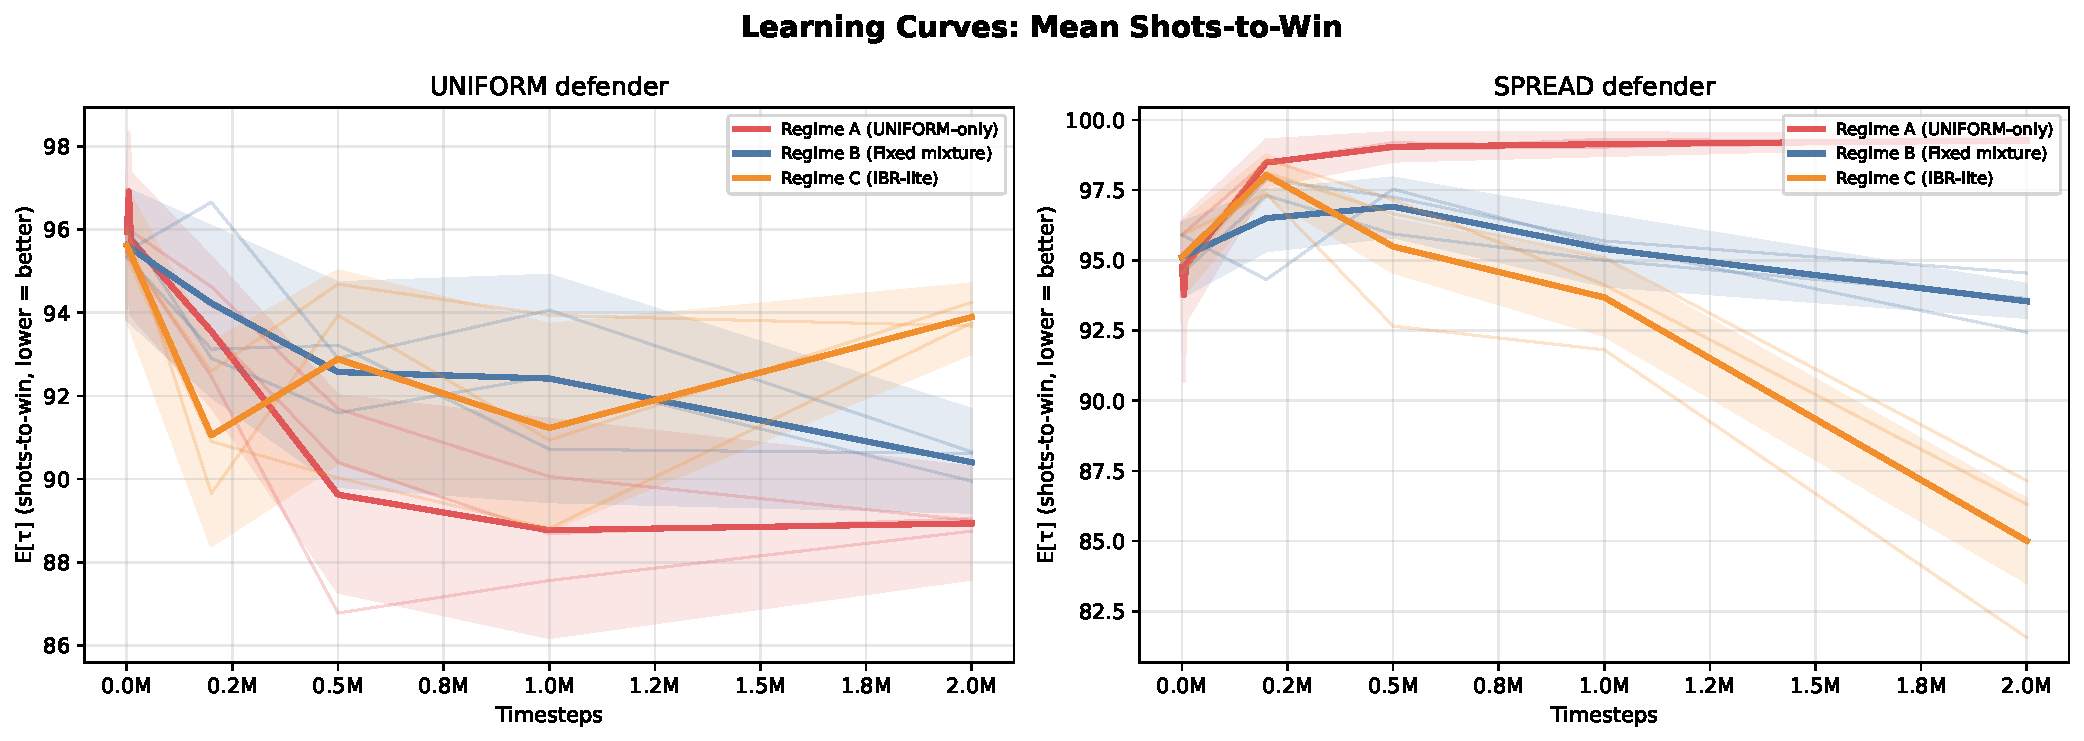
\includegraphics[width=\linewidth]{figures/fig1_learning_curves.pdf}
        \caption{Stage-1: Attacker learning curves}
        \label{fig:learning_curves}
    \end{subfigure}
    \hfill
    \begin{subfigure}[b]{0.48\linewidth}
        \centering
        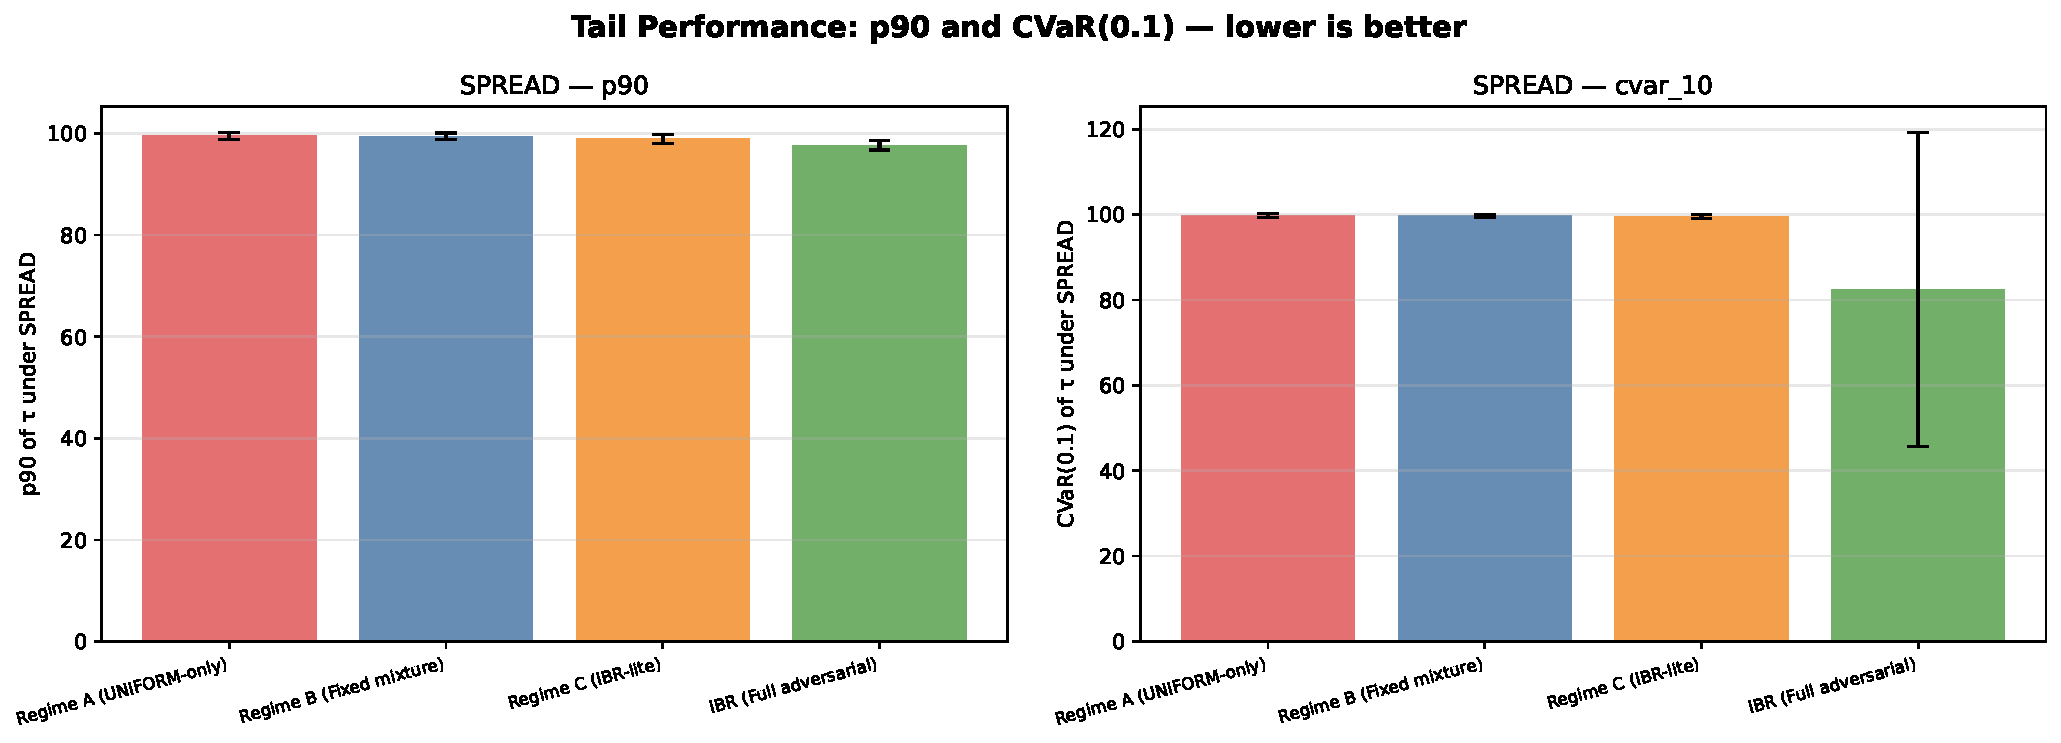
\includegraphics[width=\linewidth]{figures/fig2_tail_curves.pdf}
        \caption{Stage-1: Tail optimization curves}
        \label{fig:tail_curves}
    \end{subfigure}

    \vspace{2em}

    \begin{subfigure}[b]{0.85\linewidth}
        \centering
        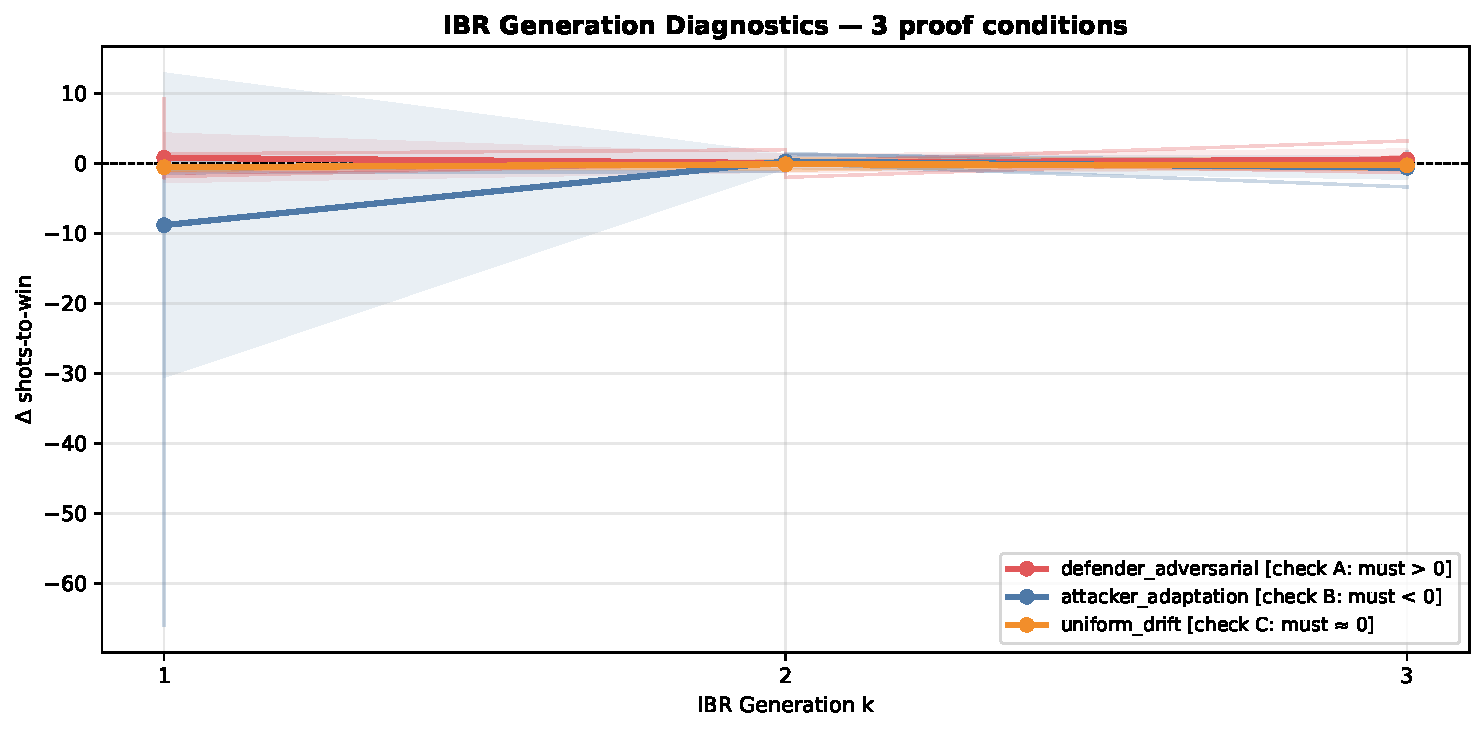
\includegraphics[width=\linewidth]{figures/fig3_ibr_generation.pdf}
        \caption{Stage-2: Final IBR generation diagnostics}
        \label{fig:ibr_generation}
    \end{subfigure}

    \caption{Training dynamics and IBR diagnostics averaged over independent seeds. \textbf{(a)} Fixed-mixture and alternating stress approaches readily acquire nominal proficiency without catastrophic gameplay degradation. \textbf{(b)} Direct targeted adversarial exposure effectively limits extreme worst-case trajectory vulnerabilities, explicitly lowering tail severity ($\cvar_{0.10}$ and $p95$). \textbf{(c)} In Stage 2, tracked IBR metrics show that sufficient optimization bandwidth can yield positive \textsf{defender\_adversarial} shifts and subsequent \textsf{attacker\_adaptation}; these curves should be read as theorem-motivated diagnostics rather than as exact row-wise certificates.}
    \label{fig:all_diagnostics}
\end{figure}
\clearpage

\bibliographystyle{unsrtnat}
\bibliography{references}

\end{document}
